\documentclass[11pt,twoside]{article}

\usepackage{paperlighter}

% Recommended, but optional, packages for figures and better typesetting:
\usepackage{microtype}
\usepackage{graphicx}
\usepackage{subfigure}
\usepackage{booktabs} % for professional tables

% Attempt to make hyperref and algorithmic work together better:
\newcommand{\theHalgorithm}{\arabic{algorithm}}


% For theorems and such
\usepackage{amsmath}
\usepackage{amssymb}
\usepackage{mathtools}
\usepackage{amsthm}

% if you use cleveref..
\usepackage[capitalize,noabbrev]{cleveref}

%%%%%%%%%%%%%%%%%%%%%%%%%%%%%%%%
% THEOREMS
%%%%%%%%%%%%%%%%%%%%%%%%%%%%%%%%
\theoremstyle{plain}
\newtheorem{theorem}{Theorem}[section]
\newtheorem{proposition}[theorem]{Proposition}
\newtheorem{lemma}[theorem]{Lemma}
\newtheorem{corollary}[theorem]{Corollary}
\theoremstyle{definition}
\newtheorem{definition}[theorem]{Definition}
\newtheorem{assumption}[theorem]{Assumption}
\theoremstyle{remark}
\newtheorem{remark}[theorem]{Remark}

% Todonotes is useful during development; simply uncomment the next line
%    and comment out the line below the next line to turn off comments
%\usepackage[disable,textsize=tiny]{todonotes}
\usepackage[textsize=tiny]{todonotes}
\usepackage{listings}

\definecolor{mygreen}{rgb}{0,0.6,0}

\lstset{
  frame=tb,
  tabsize=2,
  showstringspaces=false,
  language=C++,
  basicstyle=\footnotesize,
  captionpos=b,
  keywordstyle=\color{blue},
  stringstyle=\color{red},
  commentstyle=\color{mygreen},
  morecomment=[l][\color{green}]{\#}
}


\slimtitle{Bug Report}
%\slimauthor{Author One et al.}


\begin{document}

\lightertitle{Bug Report}
\lightersubtitle{\#402 Deadlock when running subflows in a pipeline} 
%\lighterauthor{Author One$^{\dagger}$, Author Two$^{\ddagger}$}
%
%\lighteraddress{$^\dagger$}{Address One}
%\lighteraddress{$^\ddagger$}{Address Two}


%\lighteremail{xxx@xxx.com}


%\input{content/abstract}
%\input{content/format}
%\input{content/others}


%\bibliographystyle{plainnat}
%\bibliography{ref}

%\newpage
%\appendix
%\input{content/appendix}

\section{Problem Statement}

The problem is stated in https://github.com/taskflow/taskflow/issues/402.
Listing \ref{listing::problem} shows the code.
When we spawn Subflow tasks in a pipe and call \textit{Runtime::run}
to schedule the Subflow tasks,
we run into a data race and trap in an \textcolor{red}{infinite loop}.
We print out the join counter of the scheduled runtime task in
\textit{Executor::\_invoke} and find out the value is the maximum value of size\_t.
Since a spawned Subflow task has the runtime task as its parent,
when a worker finishes a Subflow task and begins to decrement the join counter
of the parent of the finished Subflow task (runtime task),
the join counter is zero already.
Decrementing one from zero results in the maximum value of size\_t.
Now the parent node (runtime task) has a join counter of an extreme big value
but no spawned task in its queue.
There is no way to decrement its join counter to zero.
The runtime task then traps in an infinite loop 
 
\begin{lstlisting}[language=C++,label=listing::problem,caption={Code of the problem.}]
tf::Pipeline pl(
  num_lines, 
  tf::Pipe{
    tf::PipeType::SERIAL, [max_tokens](tf::Pipeflow& pf){
      if (pf.token() == max_tokens) {
        pf.stop();
      }
    }
  },

  tf::Pipe{
    tf::PipeType::PARALLEL, [&](tf::Pipeflow&, tf::Runtime& rt) mutable {
      rt.run([&](tf::Subflow& sf) mutable {
        for (size_t i = 0; i < 2; ++i) {
          sf.emplace([&](){
            ++sums;  
          });
        }
      });
    }
  }
);

\end{lstlisting}


%\begin{figure}[!h]
%  \centering
%  \centerline{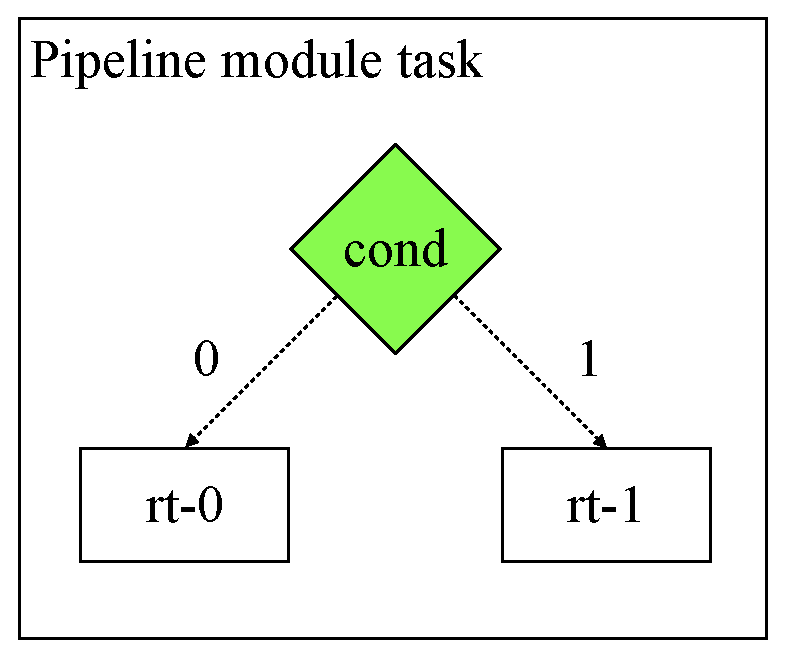
\includegraphics[width=.3\columnwidth]{Figure/pipeline_module_task.eps}}
%  \caption{
%    Our pipeline is a module task. Inside the module task, there is one condition task
%    and several runtime tasks. Here, the pipeline module task has two runtime tasks.
%    The parent of a runtime task is the pipeline module task.
%  }
%  \label{fig::pipeline_module_task}
%\end{figure}



\section{Why The Problem Exists?}

In our pipeline algorithm, we guarantee that only one worker
runs the \textit{on\_pipe} of each parallel line.
Sometimes there are two workers running on the
same parallel line.
For example, in Figure \ref{fig::pipeline} \texttt{worker j} resolves
the horizontal dependency, decrements the join counter of \texttt{C} to one.
Then \texttt{worker i} resolves the vertical dependency, decrements the
join counter of \texttt{C} to zero and calls \textit{Runtime::schedule} to schedule
\texttt{C}.
At this moment, \texttt{woker j} has not yet returned and another worker
may already start to run \textit{C}.
Then we have two workers running on the same parallel line.

\begin{figure}[!h]
  \centering
  \centerline{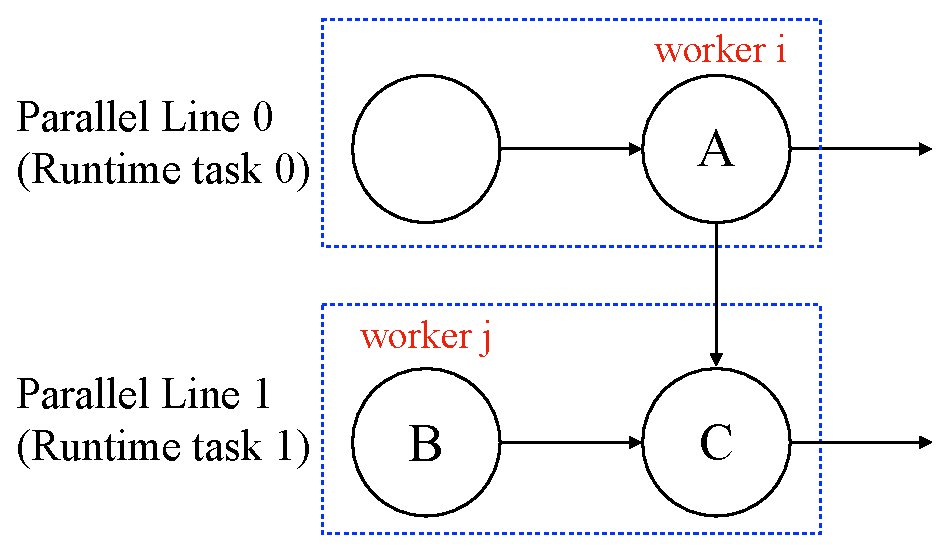
\includegraphics[width=.5\columnwidth]{Figure/pipeline.eps}}
  \caption{
    A pipeline of two parallel lines. Blue boxes depict parallel lines.
    \texttt{worker i} is running \texttt{A} and \texttt{worker j} is running \texttt{B}.
  }
  \label{fig::pipeline}
\end{figure}

Remember in our pipeline algorithm every task has two works to do in sequence.
The first part is to execute \textit{on\_pipe}
and the other part is to resolve dependency.
Although we may have two workers running on the same parallel line,
we guarantee that one worker is running the \textit{on\_pipe} and
the other worker is dealing with the scheduling.

The problem arises when a worker starts to execute \textit{on\_pipe} of \texttt{C}
and updates the join counter of runtime task 1 to the number of spawned Subflow tasks
of zero dependent.
Right after the update of the join counter by a worker,
\texttt{work j} returns and starts to reset the join counter of runtime task 1 to its
initial value. 
Since there are two workers running runtime task 1, the reset and update
of the join counter interleaves.
That is when the problem starts. 

Figure \ref{fig::illustration} illustrates the cause of the problem.
The red rectangular is supposed to run before the blue rectangular because
red rectangular represents the dependency resolving work of \texttt{B}
and the blue represents the \texttt{on\_pipe} work of \texttt{C}.
Since there are two workers running runtime task 1,
the execution order of the red and the blue boxes
can not be guaranteed.
When the blue boxes runs before the red boxes,
the join counter of runtime task 1 
are updated to two by \texttt{worker k} first.
Then the red box runs and \texttt{worker j} resets
the join counter of runtime task 1 to zero and returns to the thread pool.
Next, in the orange rectangular \texttt{worker k} finishes
one Subflow task, decrements the zero join counter of runtime task 1 by one
and gets the maximum value. An infinite loop happens.
  


\begin{figure}[!h]
  \centering
  \centerline{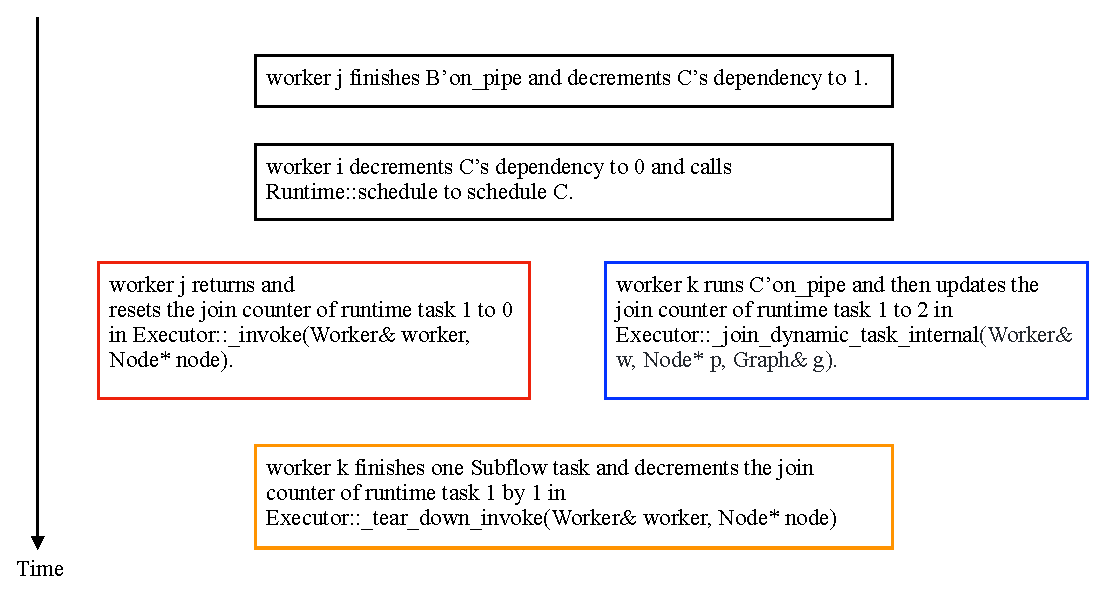
\includegraphics[width=.9\columnwidth]{Figure/illustration.eps}}
  \caption{
    Illustration of the problem when running the pipeline of Listing \ref{listing::problem}.
    The symbols align with those in Figure \ref{fig::pipeline}.
  }
  \label{fig::illustration}
\end{figure}

In conclusion, the problem arises because in our Pipeline algorithm
every parallel line could have up to two workers running simultaneously.
Although the two workers deal with different works, \texttt{on\_pipe}
and scheduling,
one worker tries to reset the join counter of the runtime task before returning,
meanwhile the other worker updates the join counter because of its spawned
Subflow tasks.
The interleaving of reset and update leads to a data race and
potentially results in an infinite loop.




\section{Solution}

To solve the problem,
in \textit{Executor::\_invoke(Worker\& worker, Node* node)},
we do not directly assign the join counter to node's initial value but
\textit{ADD} the value.
In this way,
the update of join counter in the blue rectangular in Figure \ref{fig::illustration}
is not revoked in the reset in the red rectangular
when the blue box runs before the red box.
As shown in Listing \ref{listing::solution},
we \textit{ADD} rather than assign.
 

\begin{lstlisting}[language=C++,label=listing::solution,caption={Solution to the bug.}]
if((node->_state.load(std::memory_order_relaxed) & Node::CONDITIONED)) {
  //node->_join_counter = node->num_strong_dependents();
  node->_join_counter.fetch_add(node->num_strong_dependents());
}
else {
  //node->_join_counter = node->num_dependents();
  node->_join_counter.fetch_add(node->num_dependents());
}
\end{lstlisting}






\end{document}
